\chapter{Feedforward Neural Network}

Starting from the late 2000's, neural networks have been experiencing an exciting resurgence in the big data era. Given recent improvements in processing speeds, large-scale deep neural networks (DNNs), a.k.a. deep learning, are able to deliver highly accurate results when tackling several problem domains, including computer vision, natural language processing, speech recognition, and other AI challenges. For instance, the systems using DNNs have reported breakthroughs in object recognition accuracy on the ImageNet dataset, and have even achieved human-level performance for face recognition. Motivated by these encouraging results, there has been a growing interest from both academia and industry (Google, Facebook, Amazon, etc.), both of whom have been devoted significant resources to investigate, improve and promote exploration into DNNs. DNNs are revolutionizing a number of traditional and emerging real-world applications, such as self-driving systems, automatic machine translations, drug discovery and toxicology.

In this chapter we will introduce the basics of deep feedforward neural networks, define related terminologies, and analyze how to train and use neural network model.
\section{Feedforward Networks}
A \textit{network model} is a model expressed through compositions of function, where the composition relations forms an directed acyclic graph. Figure \ref{fig1} gives an example of a network model. In this example, $f_1$ and $f_3$ are composited by $f_2$ and $f_4$ separately, which in turn is composited $f_5$. Thus the expression of the entire model is
\begin{align*}
\label{enetwork}
f(\bm{x}) = f_5(f_2(f_1(\bm{x})), f_4(f_3(\bm{x})))
\end{align*}
In a network model, the input vector is denoted as $\bm{x}\in\mathbb{R}^m$. If the information flows through the function that evaluates $\bm{x}$, through each of the subsequent function, and finally goes to output vector $\bm{y}\in\mathbb{R}^n$. Such network is called a \textit{feedforward network}, as there is no feedback connections in which outputs of the model are fed back into itself.

\begin{wrapfigure}{r}{0.3\textwidth}
\centering
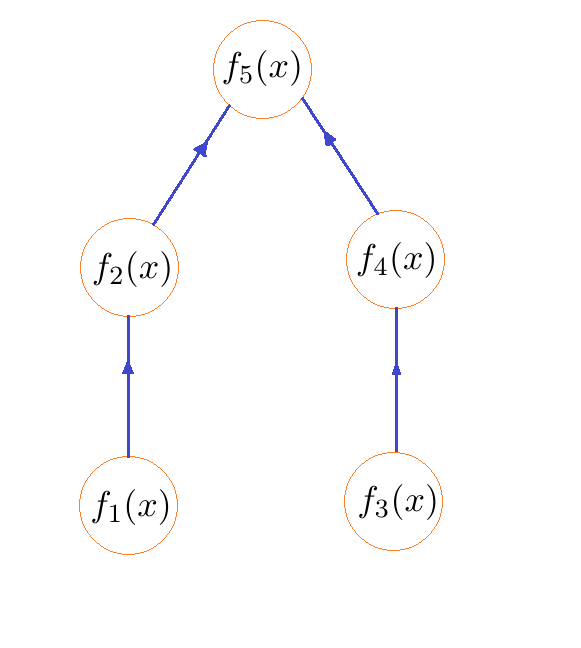
\includegraphics[width=0.3\textwidth]{Fig1}
\caption{Feedforward Network}
\label{fig1}
\end{wrapfigure}



Functions may form one or more layers according to which values they take as inputs (cf. Figure \ref{fig2}). The functions that directly take input $\bm{x}$ form the \textit{input layer}, functions that take values from input-layer functions form the \textit{first hidden layer}, and so on, until the last layer (call \textit{output layer}) which returns the output of the entire model. The total number of layers is called \textit{the depth} of the network. The \textit{width} of a layer is defined to be the number of functions on the layer. The functions are sometimes referred to as units, neurons, or activation functions, depending on the context. Nowadays neural networks with more than 1000 layers were used for tasks in computer vision, which justifies the name "deep learning". The training data do not provide information on what values the intermediate layers should produce, thus these layers are referred to as \textit{hidden layers}.

The information usually flow into a function from multiple sources. This is typically achieved by a weighted summation of the input values, possibly added with a bias value. For a single unit with activation function $\sigma$, the relation between the input vector $\bm x$ and the output vector $\bm y$ is given in the form of
\begin{equation}
    \bm y = \bm \sigma(\bm{W^Tx}+\bm\theta).
\end{equation}
Here $\bm W$ is a matrix of parameters representing the weighted summation of the input vector, $\bm\theta$ is a vector representing the bias value, and $\bm\sigma$ is the function that applies the activation function $\sigma$ to each of its input coordinates. For the ease of notation, we use new notations
$\bm x' = (\bm x^T, 1)^T$ and $\bm W' = (\bm W, \bm\theta^T)^T$ and simplify the notation above as
\begin{equation}
 \bm y = \bm \sigma(\bm{(W')^Tx'}).
\end{equation}
From now on we will drop the primes and stick with the simplified notations. As an example, the overall expression of the model illustrated in Figure \ref{fig2} can be expressed as

\begin{align*}
\bm{y} = \bm{W_3^T\cdot\sigma(W_2^T\cdot\sigma
(W_1^Tx))}
\end{align*}

The weight matrix related to the input of $j$-th layer is referred to as the weight matrix \textit{of that layer}. Every layer except for the input layer has a corresponding weight matrix.

\begin{wrapfigure}{r}{0.5\textwidth}
\centering
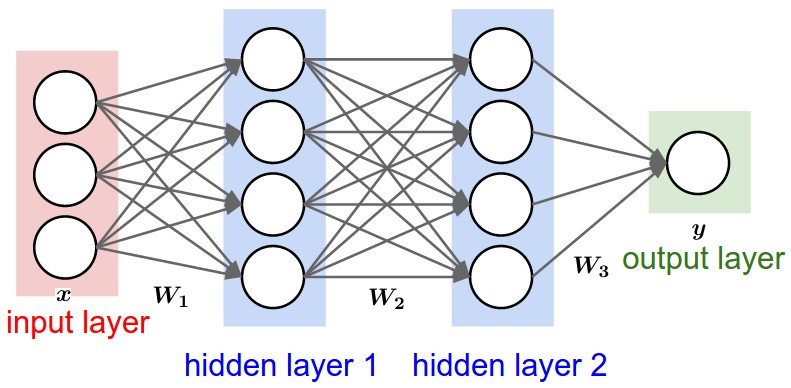
\includegraphics[width=0.5\textwidth]{Fig2}
\caption{Feedforward Network}
\label{fig2}
\end{wrapfigure}
%{\bf complicated network}
%Not every network model of interest is a layered feedforward network, as the topology of an acyclic graph can be quite complicated. Note that since there is no loop in the graph, one can still find a suitable order to let the information flow from input to output. Also there are network models that do contain directed cycles. An important class is called \textit{recurrent neural network}. We will study recurrent neural network at a later stage of the seminar.

The goal of a feedforward network is to approximate a function $g(\bm{x})$. More precisely, the goal is to find an appropriate set of weights so that the function representing the network is close to the target function $g$ (under certain measure). The challenge is to find a network model and a training method that is capable to well approximate the target function with limited memory space and computational power. The purpose the the next two sections is to introduce the basic setting of linear network models and neural network models, analyze their training procedures, and discuss the challenges of applying these models. 

\section{Linear Feedforward Neural Network}
One way to understand feedforward networks is to begin with linear models and consider how to overcome their limitations. Linear models, such as logistic regression and linear regression, are appealing because they may be fit efficiently and reliably, either in closed form or with convex optimization. On the other hand, linear models also have the obvious defect that the model capacity is limited to linear functions, so the model cannot understand the interaction between any two input variables.

{\bf Linear Regression Model}. Linear Regression is the simplest form of regression. We model our system with a linear combination of features to produce one output. That is,
\begin{equation}
  f(\bm x, \bm w) = \bm w^T\bm x
\end{equation}
Here $\bm x$ is the input vector, and $w_0$, $\bm w$ are parameters. Our task is then to find the values for the parameters that provide the best fit to our training data. One way to measure the fitness of the parameters is to calculate the least squares error (loss function) over our dataset $S = \{(\bm x^1, y^1), ..., (\bm x^N, y^N)\}$
\begin{equation}
  L(S, \bm w) = \frac{1}{2}\sum_{i=1}^N(f(\bm x^i, \bm w)-y^i)^2
\end{equation}

In order to find the best fit, we must minimize $L(S, \bm w)$. The approach using gradient descent takes the following form:
\begin{equation}
  \bm w \leftarrow \bm w-\eta\nabla_{\bm w}L(S, \bm w)
\end{equation}
The step size $\eta$ may be application-dependent. The gradient of the loss function explicitly is expressed as
\begin{equation}
  \nabla_{\bm w}L(S, \bm w) = \sum_i(\bm w^T\bm{x^i} - y^i)\bm x^i = (\bm{w^TX-y})\cdot\bm X
\end{equation}
Here $\bm X = (\bm x^1,...,\bm x^N)$ and $\bm y=(y^1,...,y^N)$.
Note that there exists a closed form solution for linear regression, thus this gradient descent method is rarely used in practice.

{\bf Logistic regression model}. Another example on linear feedforward network is logistic regression model. We model our system as
\begin{equation}
%   \tanh(\bm w^T \bm x + b), \textit{ where } \tanh(a) = \frac{1-\exp(a)}{1+\exp(a)}
\frac{1}{1+\exp(\bm w^T \bm x)}
\end{equation}
With training set $S = \{(\bm x^1, y^1), ..., (\bm x^N, y^N)\}$, the loss function is defined by the negative log-likelihood
\begin{equation}
 L(\bm w) = \sum_{i=1}^N\log(1+\exp(-y^i(\bm w^T\bm x^i)))
\end{equation}
The loss function is minimized by the gradient descent
\begin{equation}
  \bm w = \bm w-\eta\nabla_{\bm w}L(\bm w)
\end{equation}
with $\nabla_{\bm w}L(\bm w) = -\sum_{i=1}^N y^i\frac{\exp(-y^i(\bm w^T\bm x^i+b))}{1+\exp(-y^i(\bm w^T\bm x^i+b))}\bm x^i$.

The convexity of the loss function guarantees that the gradient descent algorithm will find the minimum value.

{\bf Summary}.The key elements of a network model can be summarized as follows: 
\begin{enumerate}
    \item A function representing a network structure.
    \item A loss function.
    \item An optimization algorithm that minimizes the value of the loss function.
\end{enumerate}

{\bf Limitations of Linear Network Model}. One important application of network models is the classification problem. A linear network is only capable of separating the dataset with hyperplanes. We are going to show a classical result on the limited capability of linear network models on classifying $p$ points in general position.

\begin{wrapfigure}{r}{0.4\textwidth}
\centering
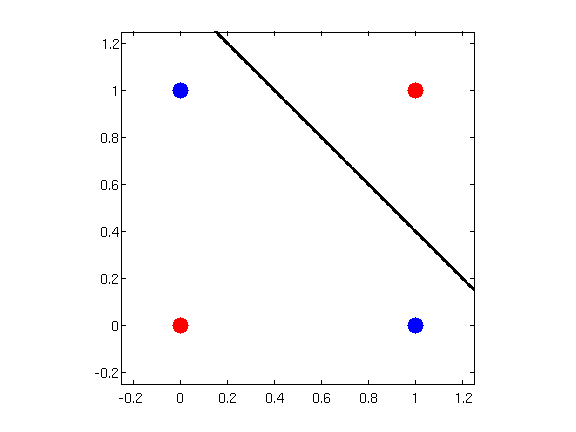
\includegraphics[width=0.4\textwidth]{nonlinearseparable}
\caption{A non-linear dichotomy}
\label{fig4}
\end{wrapfigure}

When $n$ points are partitioned into two classes, we call such classification a \textit{dichotomy}. Moreover, we use the term \textit{linearly separable dichotomies} to represent the dichotomies that are realizable by a linear classifier (the boundary between the classes is a hyperplane). Figure \ref{fig4} shows an example of a non-linear dichotomy, as no straight line can separate the two blue points from the two red ones. In general, suppose that we have $p$ points in general position in $\mathbb{R}^N$. There are $2^p$ ways to partition these $p$ points into two classes, i.e., the $p$ points can form $2^p$ different dichotomies. The following theorem shows that the proportion of linear separable dichotomies will converge to 0 as $p\rightarrow\infty$. 

% Cover's function counting theorem (1966)
% Suppose we have $p$ points in $\mathbb{R}^N$. Consider all possible partitions of these points into two classes. We have  $2^p$ such partitions. How many of there partitions yield linearly separable classes, i.e., where the two classes can be perfectly separated by an $(N-1)$-dimensional hyperplane? The only thing we assume about the points is that they are in general position, which means that any subset of $N$ or fewer points is linearly independent. 


%  A dichotomy is a partition of a whole (or a set) into two parts (subsets). In other words, this couple of parts must be jointly exhaustive: everything must belong to one part or the other, and mutually exclusive: nothing can belong simultaneously to both parts.
% Such a partition is also frequently called a bipartition.


% The two parts thus formed are complements. In logic, the partitions are opposites if there exists a proposition such that it holds over one and not the other.


% Treating continuous variables or multicategorical variables as binary variables is called dichotomization. The discretization error inherent in dichotomization is temporarily ignored for modeling purposes.

\begin{theorem}[Cover, 1965]
Let $C(p, N)$ be the number of dichotomies of $p$ points in $N$-dimensional space that can be separated by a hyperplane. Then
\begin{align*}
\lim_{p\rightarrow\infty}\frac{C(p,N)}{2^p}=0.
\end{align*}
\end{theorem}

\begin{proof}
Firstly, we will find an explicit expression for $C(p, N)$ through induction. Suppose there are $p$ points located on the plane in general position, and we are trying to add one more point. There are two possibilities:

1) There exists a separating hyperplane that passes through the new point;

2) There does not exist a separating hyperplane that passes through the new point.

In case 1), No matter which class the new point belongs to, one can always shift the hyperplane infinitesimally so that this point locates on the same side of the hyperplane with other members of the class. Thus in this case each separable partitions in $p$ points gives rise to two separable partitions in $(p+1)$ points. 

Now consider case 2). For any separating hyperplane, the new point must be on the same side with the same class of the previous $p$ points, as otherwise one can always construct a separating hyperplane that passes through the new point. Thus in this case each separable partitions in $p$ points will give rise to exactly on separable partitions in $(p+1)$ points. 

Moreover, the number of separable partitions in case 1) is equal to $C(p-1, N)$, as one degree of freedom is eliminated by requiring passing through the new point. Therefore we obtain the following recursive expression

\begin{align*}
C(p+1, N) = 2C(p,N-1) + [C(p,N)-C(p, N-1)] = C(p,N) + C(p, N-1).
\end{align*}

Moreover, we have $C(1, N)=0$ for all $N<1$ and $C(1, N)=2$ for all $N\ge 1$. By induction we can prove

\begin{align*}
C(p+1,N) = 2\sum_{i=0}^{N-1}\big(^p_i\big).
\end{align*}
Here by convention we have $\big(^p_i\big)=0$ for $p<i$.

Finally derive
\begin{align*}
&\lim_{p\rightarrow\infty}\frac{C(p,N)}{2^p}
=2\sum_{i=0}^{N-1}\lim_{p\rightarrow\infty}\frac{\big(^p_i\big)}{2^p}
=2\sum_{i=0}^{N-1}0
=0.
\end{align*}
\end{proof}

It is possible to extend linear models to represent nonlinear functions to x by applying the model to a transformed input $\phi(x)$ or with the "kernel" trick. These techniques are beyond the scope of this chapter.

\section{Feedforward Neural Network}{\color{red}LZ: merge with chapter 1}
Neural networks are a computational approach that is based on a large collection of neural units (artificial neurons), loosely mimicking the way a biological brain solves problems with large clusters of biological neurons connected by axons. Each neural unit is connected with many others, and links can be enforcing or inhibitory in their effect on the activation state of connected neural units.

Proposed in 1940$'$s, neural networks are one of the most representative models in the artificial intelligence field. Simply speaking, a neural network tries to make a system that process information as a network of human neurons. Starting from late 2000s, neural networks(NNs) have been experiencing their exciting resurgence in the emerging big data era. The technique with the use of large-size deep neural networks (DNNs), a.k.a. deep learning, have produced state-of-the-art accuracy results on several well-known datasets in different artificial intelligent tasks, such as computer vision, natural language processing, speech recognition, etc.

{\bf Sigmoid function}. The sigmoid function is defined by
\begin{equation}
\sigma(t) = \frac{1}{1+e^{-t}}.
\end{equation}
The sigmoid function is monotonically increasing over $\mathbb{R}$ and is infinitely-differentiable. It has limit 0 and 1 as $t$ approaches $+\infty$ and $-\infty$, respectively. The graph of $\sigma(t)$ is shown in Figure \ref{fsig}.

A useful property of $\sigma(t)$ is that its derivative can be expressed by the function itself.

\begin{lemma}
\label{lsig}
$\sigma'(t) = \sigma(t)(1-\sigma(t))$.
\end{lemma}


\begin{figure}\label{fsig}
\centering
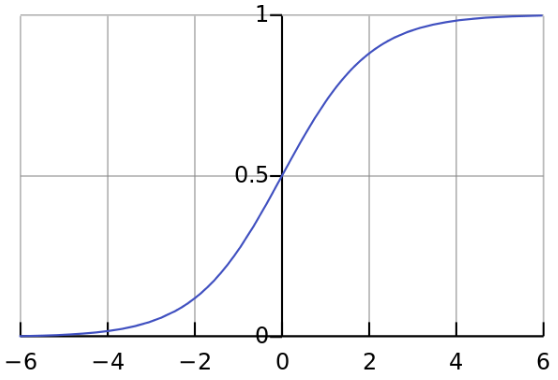
\includegraphics[width=0.3\textwidth]{Sigmoid}
\caption{Sigmoid Function}
\end{figure}

{\bf Neural network model}. In Deep Learning, sigmoid function is used as the activation function to introduce nonlinearity in the model. Inspired by biological neurons, an activation function basically works as a switch that can set the neuron on "ON" or "OFF". Besides the sigmoid function, commonly used activation functions are:

\begin{enumerate}
\item
Binary step function: $f(t) = \mathbbm{1}_{t\ge 0}$.
\item
Hyperbolic tangent function: $f(t) = tanh(t)=\frac{2}{1+e^{2t}}-1$.
\item
Arctan function: $f(t) = \tan^{-1}(t)$.
\item
Rectified linear unit (ReLU) $f(t) = max\{0, t\}$.
\end{enumerate}

A \textit{neural network} is a network model with non-linear unites on its hidden layers.

% To extend the learning model from linear to non-linear, we need to define non-linear unit, for example

% sigmoid function: expression, limits on both direction, derivative, 

% "Derivative in terms of the output y":
% \begin{align*}
% y =& \frac{1}{1+e^{-z}}\\
% \frac{dy}{dz}=&\frac{-1(-e^{-z})}{(1+e^{-z})^2}\\
% =&\big(\frac{1}{1+e^{-z}}\big)\big(\frac{e^{-z}}{1+e^{-z}}\big)\\
% =&\big(\frac{1}{1+e^{-z}}\big)\big(1 - \frac{1}{1+e^{-z}}\big)
% =y(1-y)
% \end{align*}
% %Definition of activation function. Commonly used non-linear activation function: sigmoid, tanh, ReLU, binary step:

% A activation function basically works as a switch that can set the neuron on "ON"(1) or "OFF"(0). Commonly used activation functions are:

% The first one is sigmoid function:$\sigma_1(v)=\frac{1}{1+e^{-v}}$, if $\sigma_1(v)>0.5$, we take it as an "ON", otherwise we take it as an "OFF".The second one is hyperbolic tangent:$\sigma_2(v)=tanh^{-1}(v)$, if $\sigma_2(v)>0$, we take it as an "ON", otherwise we take it as an "OFF". The third one is linear function:$\sigma_3(v)$, for linear activation function, we have the similar setting for linear function just as the previous two activation functions.



{\bf Basic neural network model.} The first thing to do when defining a machine learning model is to set the \textit{hyper-parameters}.  For a neural network, hyper-parameters include the depth of the network $d$, the width of each layer $n$, the learning rate for gradient descent $r$, and the initial values for weight matrices $(\bm{W_1}(0),...,\bm{W_d}(0))$ and biases $(\bm{\theta_1}(0),...,\bm{\theta_d}(0))$. 

 Suppose we have $m$ labeled training examples 
$$\{(\bm{x^1, y^1}),...,(\bm{x^m, y^m})\}.$$ Let $\sigma_k$ ($\bm{W_k}$, $\bm{\theta_k}$, resp.) be the activation function (weight matrix, bias vector, resp.) for the $k-th$ hidden layer, $k=1,2,...,d-1$. Let $\bm{W_d}$ and $\bm{\theta_d}$ be the weight matrix and bias vector for the output layer. 

The neural network model can be defined recursively as follows:
\begin{equation}
\label{enn}
\aligned
G_d(\bm{x}; \bm{W_1},...,\bm{W_d},\bm{\theta_1},..,\bm{\theta_d}) =& \bm{W_d^T}\bm{a_d}+\bm{\theta_d}\\
\bm{a_k} =& G_{k-1}(\bm{x}; \bm{W_1},...,\bm{W_{k-1}},\bm{\theta_1},..,\bm{\theta_{k-1}})\\
G_{k}(\bm{x}; \bm{W_1},...,\bm{W_k},\bm{\theta_1},..,\bm{\theta_k})=&
\sigma(\bm{W_k^Ta_k}+\bm{\theta_k}), k=2,...,d\\
G_1(\bm{x};\bm{W_1},\bm{\theta_1})=&\sigma(\bm{W_1^Tx}+\bm{\theta_1}).
\endaligned
\end{equation}

Here we use the convention $\sigma(x_1,...,x_n) = (\sigma(x_1),...,\sigma(x_n))$. When no confusion will occur, we will abbreviate $G_k(\bm{x}; \bm{W_1},...,\bm{W_d},\bm{\theta_1},..,\bm{\theta_d})$ as $G_k(\bm{x}; \bm{W_d},\bm{\theta_d})$ or even $G_k(\bm{x})$. 


{\bf Example: Representing XOR function}.
An \textit{XOR function} ("exclusive or") is an operation on two binary values $x_1$ and $x_2$. When exactly one of these binary values is equal to 1, the XOR function return 1. Otherwise, it returns 0. Mathematically the XOR function can be expressed as:
\begin{equation}
    f(x_1, x_2) = |x_1 - x_2|.
\end{equation}
Our model provides a function $y = f(x_1, x_2;\bm{W_1}, \bm{W_2})$ and our learning algorithm will adapt the parameters $\bm{W_1}, \bm{W_2}$ to make $f$ as similar as possible the the XOR function.
\begin{wrapfigure}{r}{0.5\textwidth}
\centering
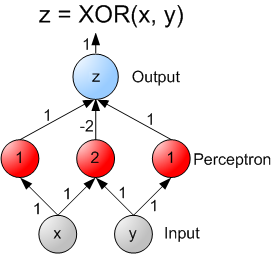
\includegraphics[width=0.25\textwidth]{XOR}
\caption{Representing XOR Function}
\label{fig3}
\end{wrapfigure}
Figure \ref{fig3} defines the network model with one hidden layer that returns exactly the same value as an XOR function on every element of the domain $\{(0,0), (0,1), (1,0), (1,1)\}$. Here the activation functions on the hidden layer are "perceptrons" $\mathbbm{1}_{x\ge a}$, where $a$ is the number inside each neuron. The expression of the neural network is
\begin{equation}
  f(x_1,x_2) = \mathbbm{1}_{x\ge 1}(x_1) -2\mathbbm{1}_{x\ge 2}(x_1+x_2) + \mathbbm{1}_{x\ge 1}(x_2).
\end{equation}
Equivalently, if we use notations 
\begin{equation}\label{exor}
    \bm x = (x_1, x_2)^T, 
    \bm{W_1} = \left[
    \begin{array}{cc}
        1 & 0 \\
        1 & 1 \\
        0 & 1 
    \end{array}
    \right],
    \bm{W_2} = \left[
    \begin{array}{c}
        1  \\
        -2 \\
        1 
    \end{array}
    \right],
\end{equation}
then equation \eqref{exor} is equivalent to the expression obtained from the general definition following equation \eqref{enn}

% Marvin Minsky and Seymour Papert (1969) showed that it was impossible for a single layer perceptron network to learn an XOR function. 
In this example, we simply specified the solution, then showed that it obtained zero error. In a real situation, there might be billions of model parameters and billions of training examples, so one cannot simply guess the solution as we did here. Instead, a gradient-based optimization algorithm can find parameters that produce very little error.

% {\bf Backpropagation}. Backpropagation is a common method of training artificial neural networks and used in conjunction with an optimization method such as gradient descent. The algorithm repeats a two phase cycle, propagation and weight update. When an input vector is presented to the network, it is propagated forward through the network, layer by layer, until it reaches the output layer. The output of the network is then compared to the desired output, using a loss function, and an error value is calculated for each of the neurons in the output layer. The error values are then propagated backwards, starting from the output, until each neuron has an associated error value which roughly represents its contribution to the original output.

% {\bf Loss function}. For backpropagation to work, two assumptions are made about the form of the error function. The first is that it can be written as an average $E = \frac{1}{n}\sum_xE_x$ over error functions $E_x$, for individual training examples, $x$. The reason for this assumption is that the backpropagation algorithm calculates the gradient of the error function for a single training example, which needs to be generalized to the overall error function. In practice, training examples are placed in batches, and the error is averaged at the end of the batch, which is then used to update the weights. The second assumption is that it can be written as a function of the outputs from the neural network.

% {\bf Example loss function}. Let $y$, $y'$ be vectors in $\mathbb R^n$. Select an error function $E(y, y')$ measuring the difference between two outputs. The standard choice is $E(y, y') = 1/2\|y-y'\|^2$. The error function over $n$ training examples can be written as an average: 
% \begin{equation}
%   E=\frac{1}{2n}\sum_x\|y(x)-y'(x)\|^2
% \end{equation}
% In order to demonstrate the idea of linear feedforward network, we give two examples 

% %Gradient computation:
% We use Back Propagation to compute the gradient of loss function $(L)$. Firstly, we have a training set by which we can train our model: Training set:$\{(x^i,y^i)|i=1,...,P\}$. Then we introduce the approximating function: $F(x)=\sigma(W^Tx+\theta)$. Namely, we use $\{(x^i, \hat{y}^i)|\hat{y}^i=F(x^i)\}$  to approximate the relationship between $x^i$ and $y^i$. After defining the approximating function, we want to compute and minimize the bias(or distance) between our approximation $\hat{y}^i$ and the real data $y^i$, so we introduce the loss function (L): L=$\frac{1}{2}\Sigma_{i=1}^{P}(y^i-\hat{y}^i)^2=\frac{1}{2}\Sigma_{i=1}^{P}(y^i-F(x^i))^2$. After this step, our work switch to minimize the loss function (L). Usually, we use gradient descent method. Thus we must compute the gradient of our loss function. Back propagation is one of the most popular method we use to compute the gradient of loss function. The essence of back propagation is just variable substitution, we set: $a=W^Tx+\theta, f=\sigma(a)$. Then the computation of gradient by back propagation is just using chain rule to compute the gradient of loss function:

% \	$\frac{\partial{L}}{\partial{f^i}}=y^i-f^i$

% \	$\frac{\partial{L}}{\partial{a}}=\frac{\partial{L}}{\partial{f^i}}\frac{\partial{f^i}}{\partial{a}}=(y^i-f^i)\sigma'(a)=(y^i-f^i)\frac{1}{cosh^2(a)}$

% %Example: approximate quadratic function:

% Implement a neural network with two layers of fully connected weights, and use it to approximate quadratic function $f(x) = x^2$.

% Firstly, we obtain the training data, that is, generate 100 values of inputs, find the corresponding function value. And then, we determine hyper-parameters, with two layers of weights, there should be one hidden layer. Decide how many neurons there should be which will depend on the amount of data.

% The third step is to initialize weights, biases, and the learning rate. After that, we come to feedforward process which is to compute the output from each input value. We use the approximating function F to give the approximating value with respect to each point in training data. Then we want to compute the gradient of our loss function in order to minimize it. We often use back propagation, the steps of back propagation is defined in the previous section. Then we repeat feedforward process and back propagation several times when loss function becomes small enough. Now the model is trained. Finally, we test our neural network by generating another set of inputs and the corresponding value of f. Compute the loss of these test values, if the results are also small, we can say that our model is well-trained.

% %Improving the performance of back-propagation:

% There are several tricks to improve the performance of back-propagation: The first one is to avoid local minima which are not the global minima of our models. For example, we can make our loss function to become a convex function which has only one minimum. The second one is to keep derivatives from going to zero, if the derivative is very small, our decent efficiency becomes very low. The third choice is to compensate for error attenuation for deep layers or reduce learning rate when weights oscillate. Next one, we prefer to use small random initial random weights and small initial learning rate to avoid "herd effect", if the learning rate is large, the loss function may grow rather than decrease after each iteration.




\section{Training a neural network model} 
{\color{red}LZ: repeated material removed}
% The error of a neural network with respect to a sample $(\bm{x},\bm{y})$ is defined by a loss function
% \begin{equation}
% \label{eloss}
% L(\bm{x}, \bm{y}; \bm{W_1},...,\bm{W_d},\bm{\theta_1},..,\bm{\theta_d}) = \frac{1}{2}\|\bm{y} - G_d(\bm{x})\|^2.
% \end{equation}

% The goal of training a neural network model is to find values for parameters $(\bm{W_1},...,\bm{W_d},\bm{\theta_1},..,\bm{\theta_d})$ such that the total loss
% \begin{equation}
% \label{etotalloss}
% L_{total}(\bm{W_1},...,\bm{W_d},\bm{\theta_1},..,\bm{\theta_d}) = \sum_{i=1}^m L(\bm{x^i}, \bm{y^i}; \bm{W_1},...,\bm{W_d},\bm{\theta_1},..,\bm{\theta_d})
% \end{equation}
% is very small. The parameters are adjusted according to $L_{total}$ using the following process called \textit{back-propagation}:
% \begin{equation}
% \label{ebp}
% \aligned
% \bm{\delta^d} =& \frac{\partial}{\partial \bm{a_d}}L_{total}(\bm{W_1},...,\bm{W_d},\bm{\theta_1},..,\bm{\theta_d})\\
% =& \sum_{i=1}^m \frac{\partial}{\partial \bm{a_d}}L(\bm{x^i}, \bm{y^i}; \bm{W_1},...,\bm{W_d},\bm{\theta_1},..,\bm{\theta_d})\\
% =& \sum_{i=1}^m \big(\bm{y^i} - G_d(\bm{x_i})\big)\\
% \bm{\delta^k} =& \frac{\partial}{\partial \bm{a_k}}L_{total}(\bm{W_1},...,\bm{W_d},\bm{\theta_1},..,\bm{\theta_d})\\
% =& \frac{\partial L_{total}}{\partial \bm{a_{k+1}}}\frac{\partial \bm{a_{k+1}}}{\partial \bm{a_k}}\\
% =& \bm{\delta^{k+1}}\bm{W_k^T}\sigma'(\bm{W_k^Ta_k}+\bm{\theta_k}), k=1,...,d-1.
% \endaligned
% \end{equation}
% For sigmoid activation function, we can apply Lemma \ref{lsig} and obtain
% \begin{equation}
% \label{ebpsig}
% \bm{\delta^k} =\bm{\delta^{k+1}}\bm{W_k^T}\circ \sigma(\bm{W_k^Ta_k}+\bm{\theta_k}) \circ (\bm{1} - \sigma(\bm{W_k^Ta_k}+\bm{\theta_k})), k=1,...,d-1.
% \end{equation}

% Here $\circ$ means element-wise multiplication of two vectors. The computation of $\bm{\delta^k}$ depends on the knowledge of $\bm{\delta^{k+1}}$, and hence the name back-propagation. The gradient of the loss function with respect to each parameter can be computed as follows: for each $k=1,...,d$ we have
% \begin{equation}
% \label{ebpparam}
% \aligned
% \frac{\partial}{\partial \bm{W_k}}L_{total}(\bm{W_1},...,\bm{W_d},\bm{\theta_1},..,\bm{\theta_d}) =& \frac{\partial}{\partial G_k}L_{total}(\bm{W_1},...,\bm{W_d},\bm{\theta_1},..,\bm{\theta_d})\bm{a_k}=\bm{\delta^k}\bm{a_k}\\
% \frac{\partial}{\partial \bm{\theta_k}}L_{total}(\bm{W_1},...,\bm{W_d},\bm{\theta_1},..,\bm{\theta_d}) =& \frac{\partial}{\partial G_k}L_{total}(\bm{W_1},...,\bm{W_d},\bm{\theta_1},..,\bm{\theta_d}) = \bm{\delta^k}
% \endaligned
% \end{equation}
% Here $G_0 = \bm{x}$. To obtain the expression in \eqref{ebpparam} we use the following properties of matrix differentiation
% \begin{equation}
% \label{ediff}
% \aligned
% \frac{\partial }{\partial \bm{A}}L(\bm{Ax + b}) =& \frac{\partial L}{\partial \bm{Ax + b}}\bm{X}\\
% \frac{\partial }{\partial \bm{b}}L(\bm{Ax + b}) =& \frac{\partial L}{\partial \bm{Ax + b}}
% \endaligned
% \end{equation}
% (Add proof)

% With the gradients computed, we use the following update rule to adjust the parameters: for $k=1,...,d,$
% \begin{equation}
% \label{ebpup}
% \aligned
% \bm{W_k} =& \bm{W_k} - r\frac{\partial L_{total}}{\partial \bm{W_k}}\\
% \bm{\theta_k} =& \bm{\theta_k} - r\frac{\partial L_{total}}{\partial \bm{\theta_k}}
% \endaligned
% \end{equation}
{\bf Complexity} The arithmetic complexity of the back-propagation process is dominated by the matrix multiplication in \eqref{ebp}. In practise variations of this algorithms such as \textit{stochasitc gradient descent} (SGD) is used to avoid large-scale matrix multiplication.

%\section{A Back-Propagation Example}
%We have seen a perceptron network with one hidden layer that represents the XOR function. In that case we hand-picked values for each parameter, while in practice a gradient-based optimization algorithm need to be applied. Here let's look at an example of finding a sigmoid network that approximate the XOR function.
%
%{\bf XOR function}. Recall that the XOR ("exclusive or") function $f^*(x_1,x_2)$ takes two binary values $x_1$ and $x_2$ as input. Thus the domain of $f^*$ is $\{(0,0),(0,1),(1,0),(1,1)\}$. When exactly one of $(x_1,x_2)$ is equal to 1, the function returns 1. Otherwise, it returns 0.
%
%For the learning of XOR function, we are going to use a neural network with two input units, one hidden layer with three sigmoid units, and one output unit. Additionally, the hidden layer and the output layer will include a bias. The weights and biases are usually initialized with random values. Here for the ease of illustration we set the initial values as:
%
%\begin{equation}
%\bm{W_1} = \left[
%\begin{array}{ccc}
%0.1 & 0.2 & 0.3\\
%0.4 & 0.5 & 0.6
%\end{array}
%\right]
%,
%\bm{W_2} = \left[
%\begin{array}{c}
%0.1\\
%0\\
%-0.1
%\end{array}
%\right]
%,
%\bm{\theta_1}= \left[
%\begin{array}{c}
%0.1\\
%0.1\\
%0.1
%\end{array}
%\right]
%,
%\bm{\theta_2} = 0.1.
%\end{equation}
%
%Note that in practice, the initial values for parameters are usually determined from a Gaussian distribution (possibly with normalization). This neural network model can be expressed mathematically as
%
%\begin{equation}
%\bm{y} = \bm{W_2^T}\sigma(\bm{W_1^Tx}+\bm{\theta_1})+\bm{\theta_2}
%\end{equation}
%
%{\bf The forward pass.} For each input tuple from $\{(0,0),(0,1),(1,0),(1,1)\}$, we calculate the output value (by convention $\sigma((x_1, ...,x_n)^T)=(\sigma(x_1),... \sigma(x_n))^T)$)
%\begin{enumerate}
%\item
%input: $\bm{x} = (0,0)^T$.
%Hidden layer:
%\begin{equation}
%\aligned
%\bm{a} =& \bm{W_1^Tx}+\bm{\theta_1} = (0.1,0.1,0.1)^T\\
%\bm{b} =& \sigma(\bm{a}) = (0.525,0.525,0.525)^T
%\endaligned
%\end{equation}
%Output layer:
%\begin{equation}
%\bm{y} = \bm{W_2^Tb}+\bm{\theta_2} = 0.1
%\end{equation}
%
%\item
%input: $\bm{x} = (0,1)^T$.
%Hidden layer:
%\begin{equation}
%\aligned
%\bm{a} =& \bm{W_1^Tx}+\bm{\theta_1} = (0.5,0.6,0.7)^T\\
%\bm{b} =& \sigma(\bm{a}) = (0.622,0.646,0.668)^T
%\endaligned
%\end{equation}
%
%Output layer:
%\begin{equation}
%\bm{y} = \bm{W_2^Tb}+\bm{\theta_2} = 0.0954
%\end{equation}
%
%\item
%input: $\bm{x} = (1,0)^T$.
%Hidden layer:
%\begin{equation}
%\aligned
%\bm{a} =& \bm{W_1^Tx}+\bm{\theta_1} = (0.2,0.3,0.4)^T\\
%\bm{b} =& \sigma(\bm{a}) = (0.550,0.574,0.599)^T
%\endaligned
%\end{equation}
%
%Output layer:
%\begin{equation}
%\bm{y} = \bm{W_2^Tb}+\bm{\theta_2} = -0.0951
%\end{equation}
%\item
%input: $\bm{x} = (1, 1)^T$.
%Hidden layer:
%\begin{equation}
%\aligned
%\bm{a} =& \bm{W_1^Tx}+\bm{\theta_1} = (0.6,0.8,1.0)^T\\
%\bm{b} =& \sigma(\bm{a} = (0.646,0.690,0.731)^T
%\endaligned
%\end{equation}
%
%Output layer:
%\begin{equation}
%\bm{y} = \bm{W_2^Tb}+\bm{\theta_2} = 0.0914
%\end{equation}
%\end{enumerate}
%
%{\bf Calculating the total error.} The set of inputs and outputs for XOR function includes
%\begin{align*}
%    \bm x^1 =& (0,0)^T, y^1 = 0\\
%    \bm x^2 =& (0,1)^T, y^2 = 1\\
%    \bm x^3 =& (1,0)^T, y^3 = 1\\
%    \bm x^4 =& (1,1)^T, y^4 = 0
%\end{align*}
%The expression for the neural network model is
%\begin{equation}
%G(\bm x; \bm W_1, \bm W_2, \bm \theta_1, \bm \theta_2) = \bm W_2^T\sigma(\bm W_1^T+\bm\theta_1)+\bm\theta_2.
%\end{equation}
%We can now calculate the error for each output neuron using the squared error function and sum them to get the total error:
%\begin{equation}
%L(\bm x; \bm W_1, \bm W_2, \bm \theta_1, \bm \theta_2) = \frac{1}{2}\sum_i (\bm{y^i} - G(\bm x^i; \bm W_1, \bm W_2, \bm \theta_1, \bm \theta_2))^2= 0.828
%\end{equation}
%
%Here the sum is over all four possible inputs. Note that The $\frac{1}{2}$ is included so that exponent is canceled when we differentiate later on. The result is eventually multiplied by a learning rate anyway so it doesn't matter that we introduce a constant here.
%
%{\bf The Backward Pass}
%Our goal with back-propagation is to update each of the weights in the network so that they cause the actual output to be closer the target output, thereby minimizing the error for each output neuron and the network as a whole.
%
%\begin{enumerate}
%\item
%Loss function: $L = 1/2\sum_i(\bm{y^i} - G(\bm{x^i}))^2$
%\begin{equation}
%\frac{\partial L}{\partial \bm{y}} = \sum_i \bm{y^i} - G(\bm{x^i}) = 0.0915
%\end{equation}
%\item
%Output layer: $\bm{y} = \bm{W_2^Tb}+\bm{\theta_2}$, $\bm{b} = \sigma(\bm{a})$
%\begin{equation}
%\aligned
%\frac{\partial L}{\partial \bm{W_2}} =& \bm{b}\big(\frac{\partial L}{\partial \bm{y}}\big)^T = \left[
%\begin{array}{c}
%-0.949\\
%-0.988\\
%-1.027
%\end{array}
%\right]
%\\
%\frac{\partial L}{\partial \bm{b}} =& \bm{W_2}\big(\frac{\partial L}{\partial \bm{y}}\big)=\left[
%\begin{array}{c}
%0.00915\\
%0     \\
%0.00915
%\end{array}
%\right]\\
%\frac{\partial L}{\partial \bm{\theta_2}} =& \frac{\partial L}{\partial \bm{y}}=-1.618\\
%\frac{\partial L}{\partial \bm{a}} =& \frac{\partial L}{\partial \bm{b}}\circ \sigma'(\bm{a}) = \frac{\partial L}{\partial \bm{b}}\circ \bm{b} \circ (\bm{1}-\bm{b})
%=\left[
%\begin{array}{c}
%0.0032\\
% 0.0002      \\
%-0.0022
%\end{array}
%\right]
%\endaligned
%\end{equation}
%Here $\circ$ represents element-wise multiplication, and $\bm{1}$ represents the vector with all coordinate equal to 1.
%\item
%Hidden layer:
%\begin{equation}
%\aligned
%\frac{\partial L}{\partial \bm{W_1}} =& \bm{x}\big(\frac{\partial L}{\partial \bm{a}}\big)^T = \left[
%\begin{array}{ccc}
%-0.0203 & 0        &  0.0199\\
%-0.0191 & 0        &  0.0182
%\end{array}
%\right]\\
%%\frac{\partial L}{\partial \bm{x}} =& \bm{W_1}\big(\frac{\partial L}{\partial \bm{a}}\big)\\
%\frac{\partial L}{\partial \bm{\theta_1}} =& \frac{\partial L}{\partial \bm{a}}=\left[
%\begin{array}{c}
%0.00209\\
%0\\
%-0.00180
%\end{array}
%\right]
%\endaligned
%\end{equation}
%\item
%Update parameters: fix learning rate $r = 0.01$
%\begin{equation}
%\aligned
%\bm{W_1} =& \bm{W_1} - r\frac{\partial L}{\partial \bm{W_1}}\\
%\bm{W_2} =& \bm{W_2} - r\frac{\partial L}{\partial \bm{W_2}}\\
%\bm{\theta_1} =& \bm{\theta_1} - r\frac{\partial L}{\partial \bm{\theta_1}}\\
%\bm{\theta_2} =& \bm{\theta_2} - r\frac{\partial L}{\partial \bm{\theta_2}}
%\endaligned
%\end{equation}
%\end{enumerate}
%
%After 30000 iterations, the total loss will drop to $6.97\times 10^{-9}$. See Figure \ref{fbp} for how the loss drops as iteration goes on.
%\begin{figure}[H]
%\label{fbp}
%\centering
%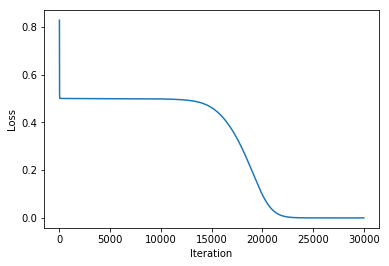
\includegraphics[scale=0.5]{Backpropfig}
%\caption{Total Loss after Each Iteration}
%\end{figure}
%
%The parameters now take values:
%\begin{equation}
%\bm{W_1} = \left[
%\begin{array}{ccc}
%1.070 & 1.055 & 3.465\\
%1.052 & 1.091 & 3.524
%\end{array}
%\right]
%,
%\bm{W_2} = \left[
%\begin{array}{c}
%-2.355\\
%-2.349\\
%3.488
%\end{array}
%\right]
%,
%\bm{\theta_1}= \left[
%\begin{array}{c}
%-1.208\\
%-1.233\\
%-0.650
%\end{array}
%\right]
%,
%\bm{\theta_2} = -0.125.
%\end{equation}
%And for each input the neural network will return:
%\begin{equation}
%\aligned
%(0,0)\mapsto 0.00004\\
%(0,1)\mapsto 0.99994\\
%(1,0)\mapsto 0.99994\\
%(1,1)\mapsto 0.00008
%\endaligned
%\end{equation}
